%.-------------------------------------------------------------------------------------------------------------------------------------------------------------
\subsection{External Interface Requirements}
%.-------------------------------------------------------------------------------------------------------------------------------------------------------------
\subsubsection{User Interfaces}


\begin{figure}[h]
\centering
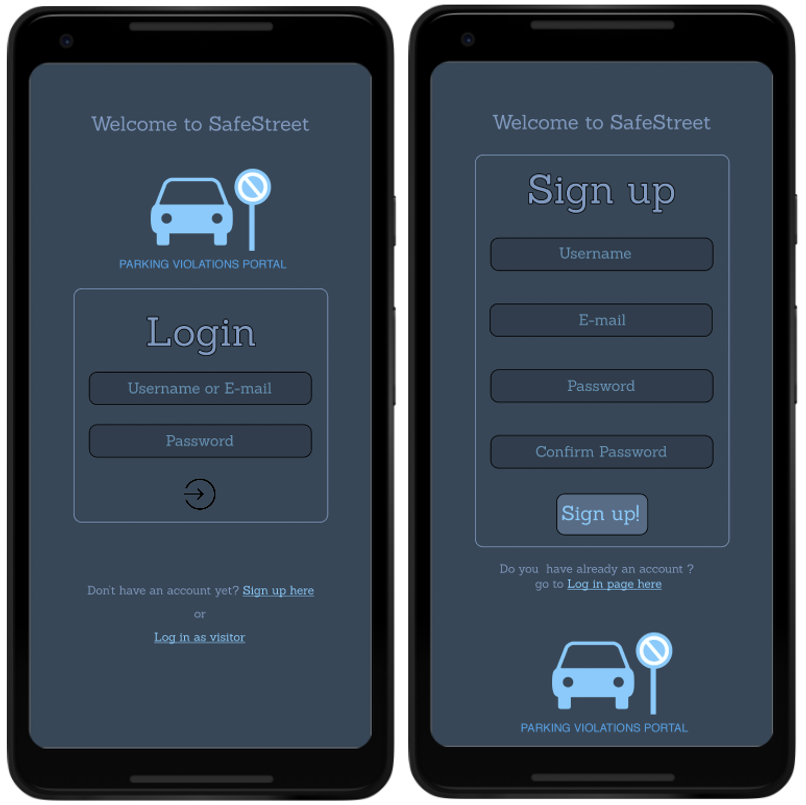
\includegraphics[width=\textwidth]{Images/login_signup.png}
\caption{\label{fig:ls}Login and Sign up }
\end{figure}

\begin{figure}[h]
\centering
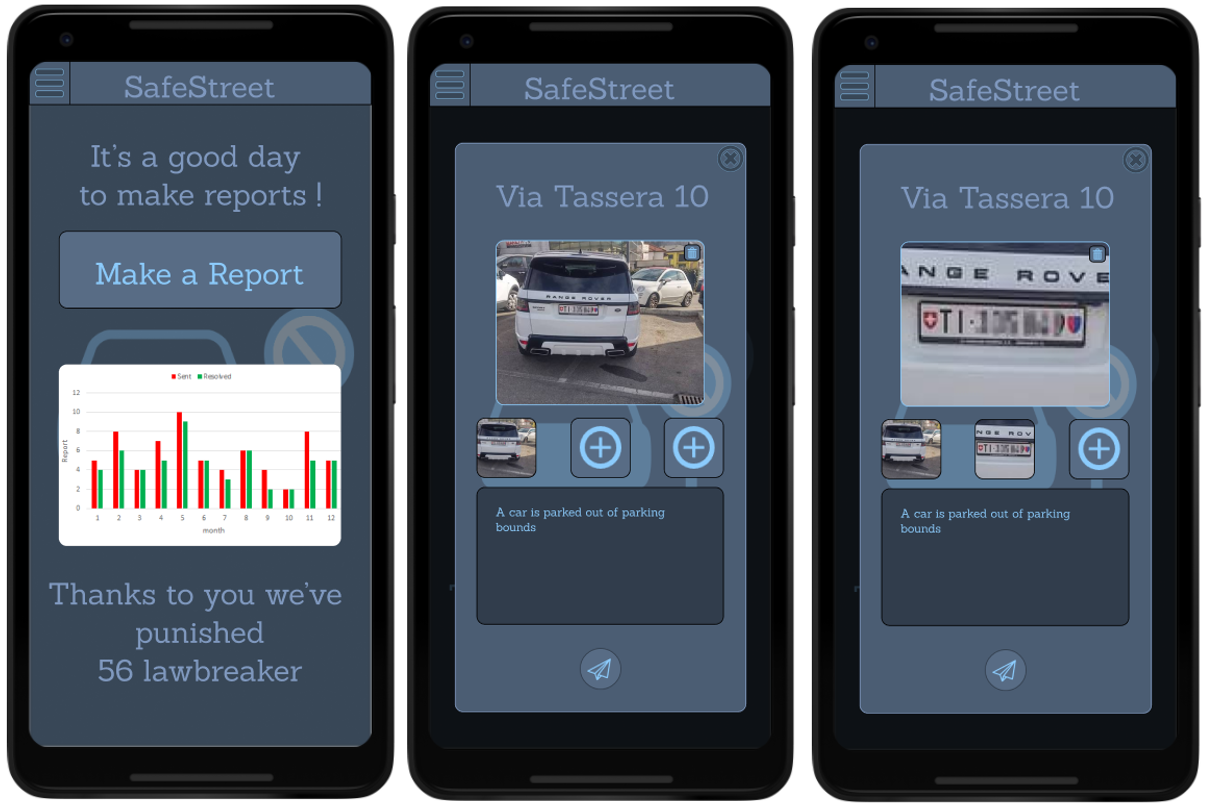
\includegraphics[width=\textwidth]{Images/user_interface.png}
\caption{\label{fig:CI}Citizen Interfaces}
\end{figure}

\begin{figure}[h]
\centering
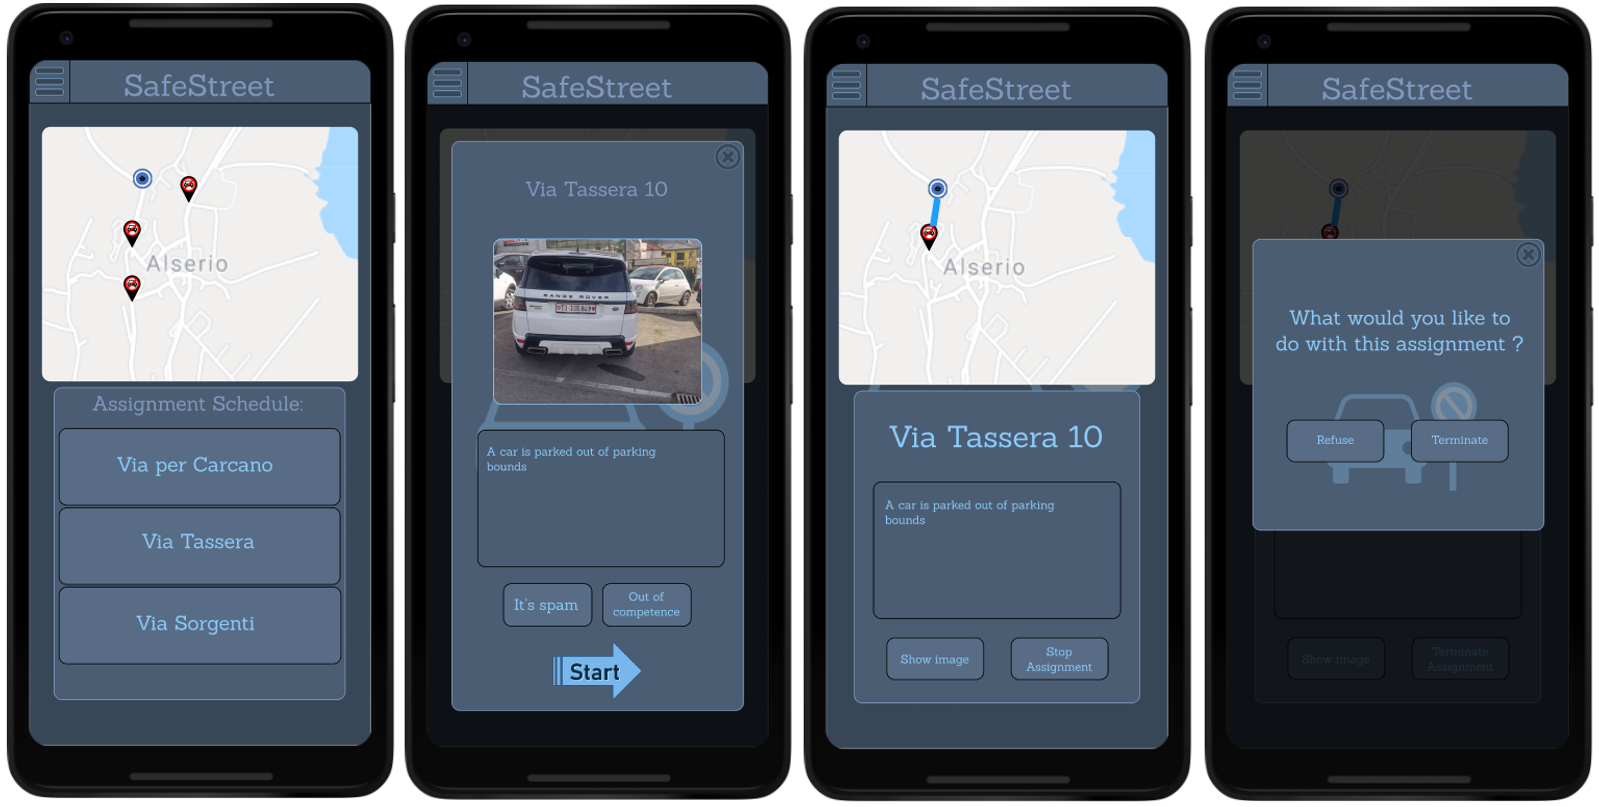
\includegraphics[width=\textwidth]{Images/agent_interface.png}
\caption{\label{fig:AI}Authority Interfaces }
\end{figure}

\begin{figure}[h]
\centering
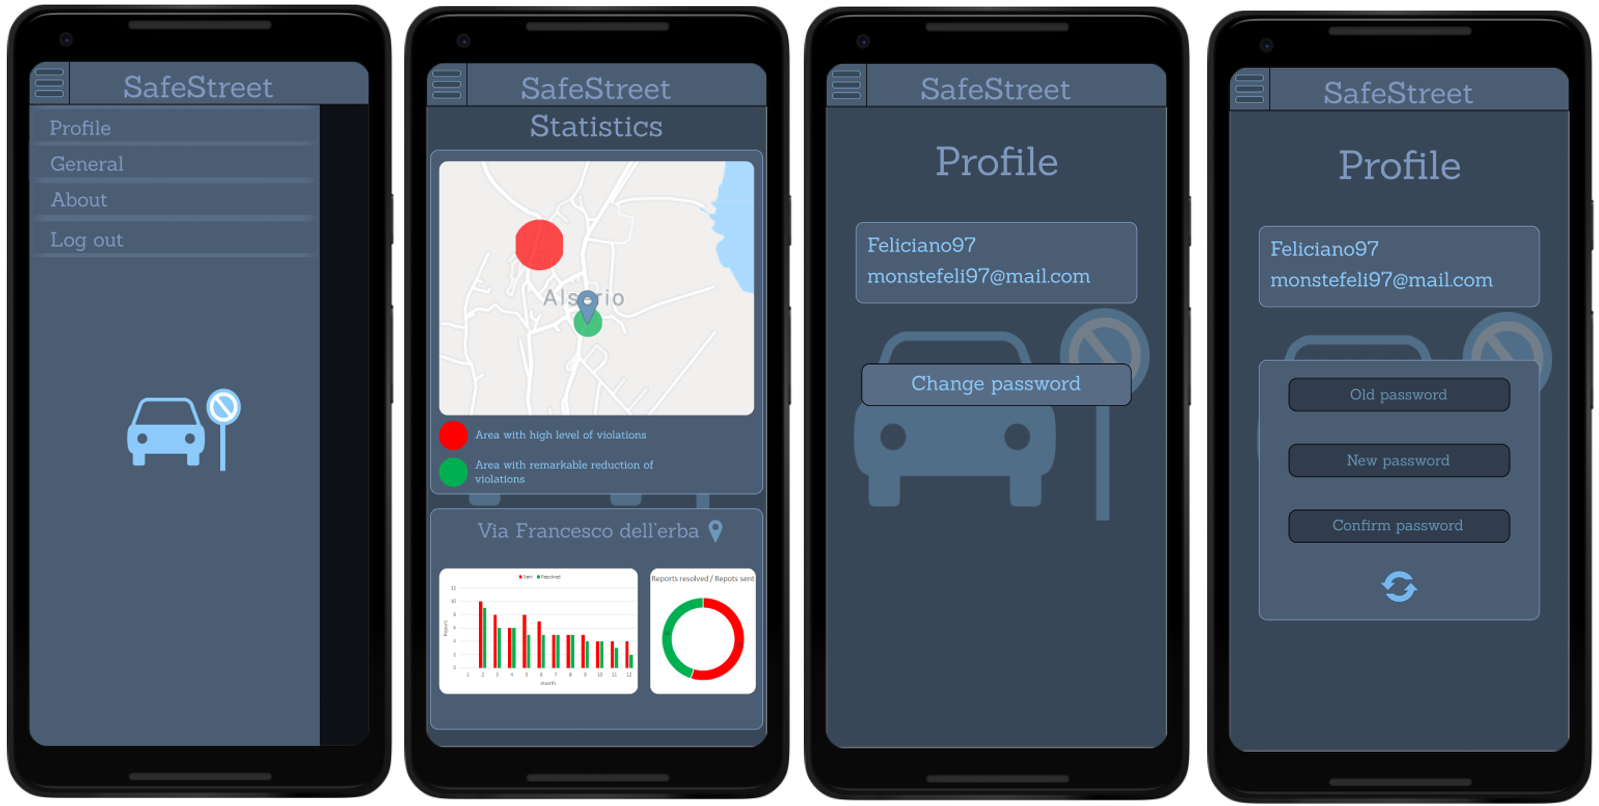
\includegraphics[width=\textwidth]{Images/common_interface.png}
\caption{\label{fig:ComI}Common Interfaces }
\end{figure}

\begin{figure}[h]
\centering
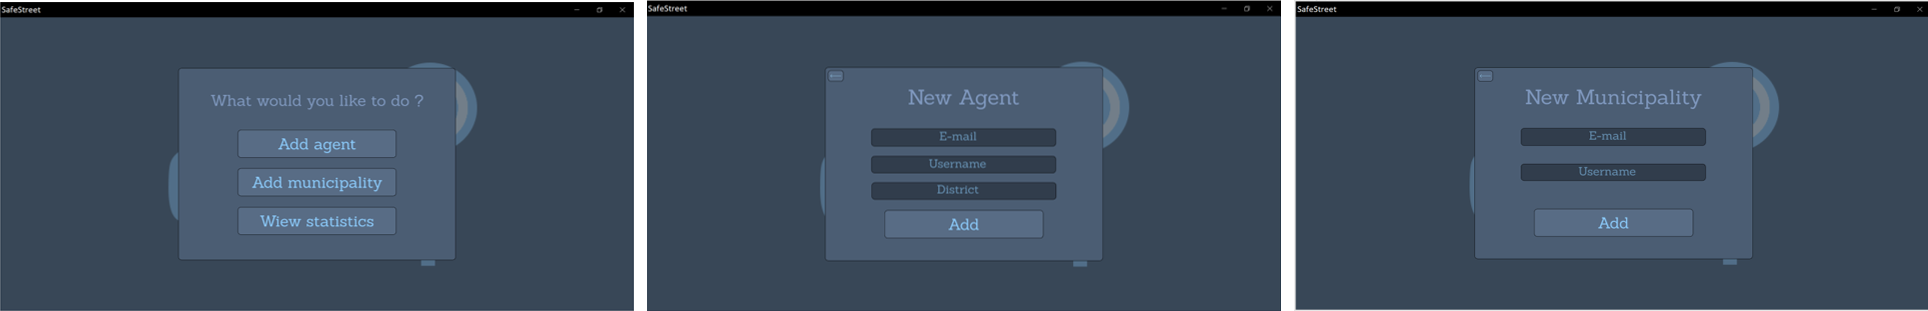
\includegraphics[width=\textwidth]{Images/municipality_interface.png}
\caption{\label{fig:MI}Municipality Interfaces }
\end{figure}

\begin{figure}[h]
\centering
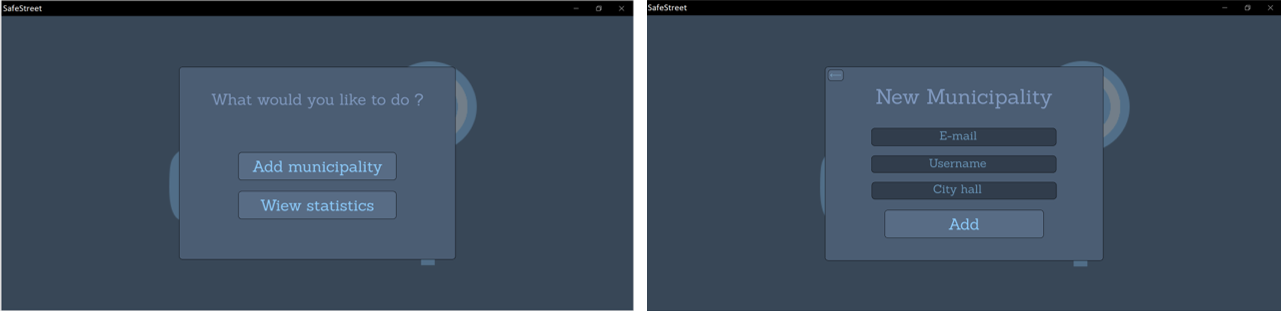
\includegraphics[width=\textwidth]{Images/system_manager_interface.png}
\caption{\label{fig:SMI}Sytem Manager Interfaces}
\end{figure}

\begin{figure}[h]
\centering
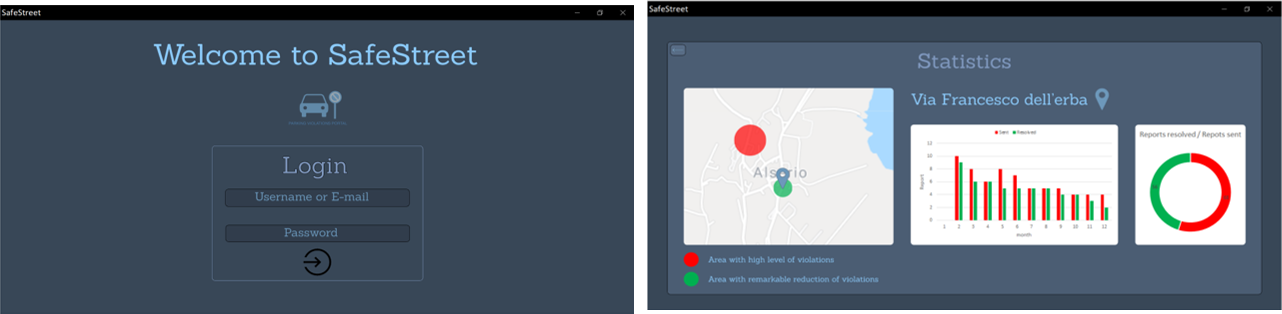
\includegraphics[width=\textwidth]{Images/desktop_common_interface.png}
\caption{\label{fig:ComWI}Common web Interfaces}
\end{figure}

%.-------------------------------------------------------------------------------------------------------------------------------------------------------------
\subsubsection{Hardware Interfaces}
There are no hardware interfaces to be implemented
%.-------------------------------------------------------------------------------------------------------------------------------------------------------------
\subsubsection{Software Interfaces}
Software interfaces to communicate with mapping systems, municipality databases and the algorithm to read Lisence plates are needed 
%.-------------------------------------------------------------------------------------------------------------------------------------------------------------
\subsubsection{Communication Interfaces }
To communicate the various internal parts of the S2B use HTTP and HTTPS protocol. No specific communication interface must be implemented.
%.-------------------------------------------------------------------------------------------------------------------------------------------------------------
\subsection{Functional Requirements}
\begin{itemize}

 \item R1) Authorities’ location must be known by the system when they are in service.
\item  R2) When a Citizen makes a report the position is correctly added with the GPS when is available.
\item R3) The right authorities are notified about violations.
 \item R4)  Authority must be able to provide the system how the assignment finished: resolved and the type of violation, no intervention needed when arrived, false report.
 \item R5) The system must make Statistics available when asked.
 \item R6) Statistics are always updated when an event happens.  
\item R7) For registering a Municipality his/hers data must be provided to a System manager who will add those data to the service to sign up him/her.
 \item R8) A visitor must be able to begin sign up process in the SafeStreets App filling a form with his data.
 \item R9) When the creation of an account is successful the system must notify the Visitor sending an email to the address provided in the sign up process. 
 \item R10) When GPS is not available the user can input the position from a map.
 \item R11) Users must be able to login if they provide the right credentials.
\item R12) The camera of the mobile phone must be accessible to take photos of violations.
\item R13) Suggestions must be available when municipalities requests them.
\item R14) The User must be able to select the licence plate between the ones in output from the Licence Plate Recognition algorithm.
\item R15) Each Username is unique
\end{itemize}
%.-------------------------------------------------------------------------------------------------------------------------------------------------------------
\subsubsection{Scenrarios}
\begin{itemize}
\item Scenario 1:
\newline
Dimitri has an important appointment, but in front of his underground garage there is a car parked that doesn’t allow him to go out. He doesn’t know who the car owner is, so he can’t call him to move it. So, Dimitri decides to use Safestreet application: he takes a photo of the car, he adds the notes and he insert manually the position, because the GPS can’t take correctly the position, in order to send the violation to the authorities. After 10 minutes the public security agent, who has received the notification of Dimitri’s alert, arrives and means of removal take the car away and finally Dimitri can go to the appointment.


\item Scenario 2:
\newline
Angelo is the town councilman of Alserio. In the last period some citizen has alerted him that there are some people who park their car in the disabled parking near the Enigma café. They also have complained about the fact that there is not a public security agent to control the area. So, Angelo asks the mayor to use SafeSteets application in order to keep the violations under control. The mayor, enthusiast of his suggestion asks the system manager to add him into the service.After that, the mayor adds the other municipality employees, so they can add the authorities too.Therefore , thanks to the app , the authorities receive warnings about infractions in various part of the town and they can intervene. Moreover, thanks to the statistics supplied by the application, the mayor manages to start a policy of prevention of the violation.
\item Scenario 3
\newline
Manuel asks his friend Fred if he wants to join him for dinner this evening at his place. Unfortunately, Fred's car is blocked by a vehicle parked in front of his garage. He has noticed that car has been there several days in the past months. Since Fred works near his house, he goes to work by bike, but his friend lives far from his house, so he can't get there without his car. So, Fred decides to download SafeStreets app on his smartphone. He provides all the information required to the system in order to sign up; then he logs in and sends a notification to the authorities. One hour before leaving he notices that the car has been removed. From that day on the car owner stopped parking there.
\item Scenario 4:
\newline
Today in Milan there are lot of violations and the authorities can't check every one of them. After some time, the violations not assigned lose their priority and go down in the assignment list. Agent Carlo usually checks the areas between Milano Piola and Milano Lambrate. Lots of violations are notified by users in those areas. However, by the time he finishes checking some violations, other become less visible due to the great amount of notifications. When different users notify a violation concerning a license plate in the same area, this one becomes more visible in the assignment list. Thanks to this feature, Carlo is able to first address issues affecting more people.

\item Scenario 5:
\newline
Pietro is an agent who has just been employed in Alserio police; his method of street controlling is “old school” and a little bit disorganized, but his colleague Sonia recommends him SafeStreet application. So, Pietro goes to the town hall to register himself into the Safestreet database. The employee checks his credential and his work district, and the system sends him the transient credential.  Then, Pietro installs the app and uses the transient credentials in order to log into his personal page and change the credentials to confirm the account. Thanks to SafeStreet application, his job is now organized better because he can go to exact violations place.
\item  Negative Use Scenario 6:
\newline
Fernand got his car fined after having parked in a forbidden area. He has been doing it for years, but now he notices that people in that area started using SafeStreets app and thinks that he was fined because of it instead of his behaviour. He decides to "take revenge" subscribing to the app and sending several false notifications. Since he has sent several random photos without any visible licence plate, the system signs the assignments given by Fernand account as "possibly unsafe". After that some agents have checked that no violation is actually in any of the photos sent to the system, his account gets blocked and Fernand can no longer interfere with the normal activities of authorities using the app. After being blocked, Fernand stops complaining about the app and a week later he finds a parking area to replace his former parking spot.
\end{itemize}
%.-------------------------------------------------------------------------------------------------------------------------------------------------------------
\newpage
\subsubsection{Use Case Diagrams}
\begin{figure}[h]
\centering
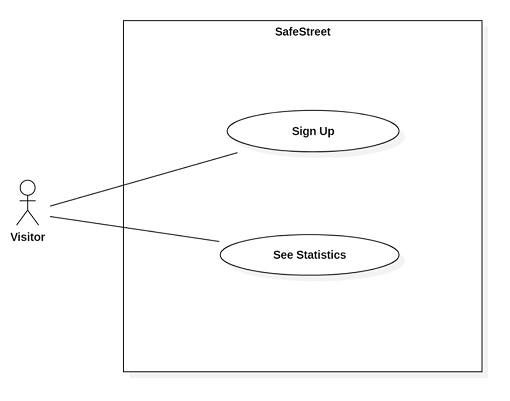
\includegraphics{Images/usecase_visitor.png}
\caption{\label{fig:VUC}Visitor Use Case }
\end{figure}
\begin{figure}[h]
\centering
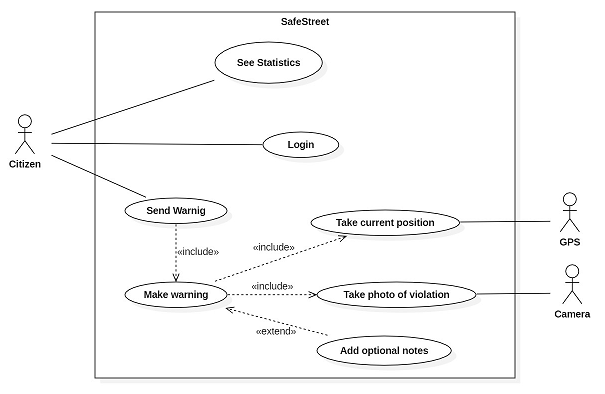
\includegraphics[width=\textwidth]{Images/usecase_citizen.png}
\caption{\label{fig:CUC}Citizen Use Case }
\end{figure}
\begin{figure}[h]
\centering
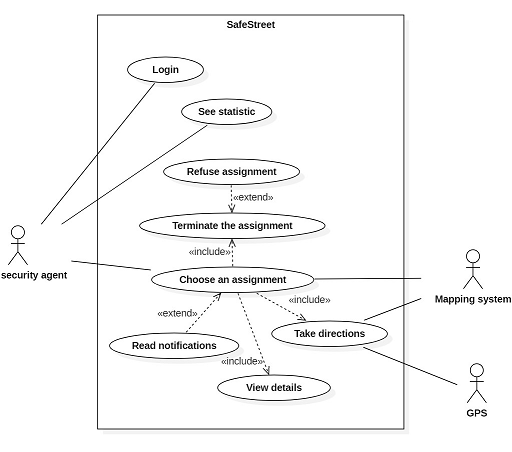
\includegraphics{Images/usecase_agent.png}
\caption{\label{fig:AUC}Authority Use Case }
\end{figure}
\begin{figure}[h]
\centering
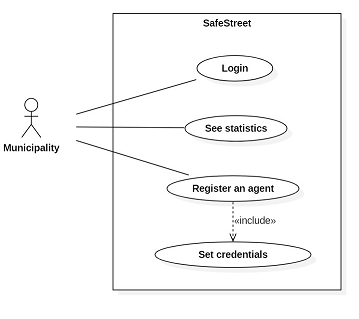
\includegraphics{Images/usecase_municipality.png}
\caption{\label{fig:MUC}Municipality Use Case }
\end{figure}
\begin{figure}[h]
\centering
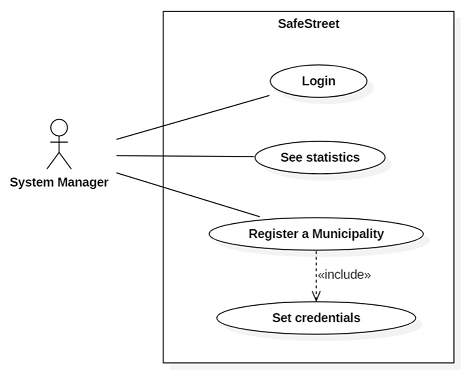
\includegraphics{Images/usecase_system_manager.png}
\caption{\label{fig:SMUC}System Manager Use Case }
\end{figure}
%.--------------------------------------------------------------------------------------------------------------------------------------------------------------
\subsubsection{Use Case Descriptions}
\begin{figure}[h]
\centering
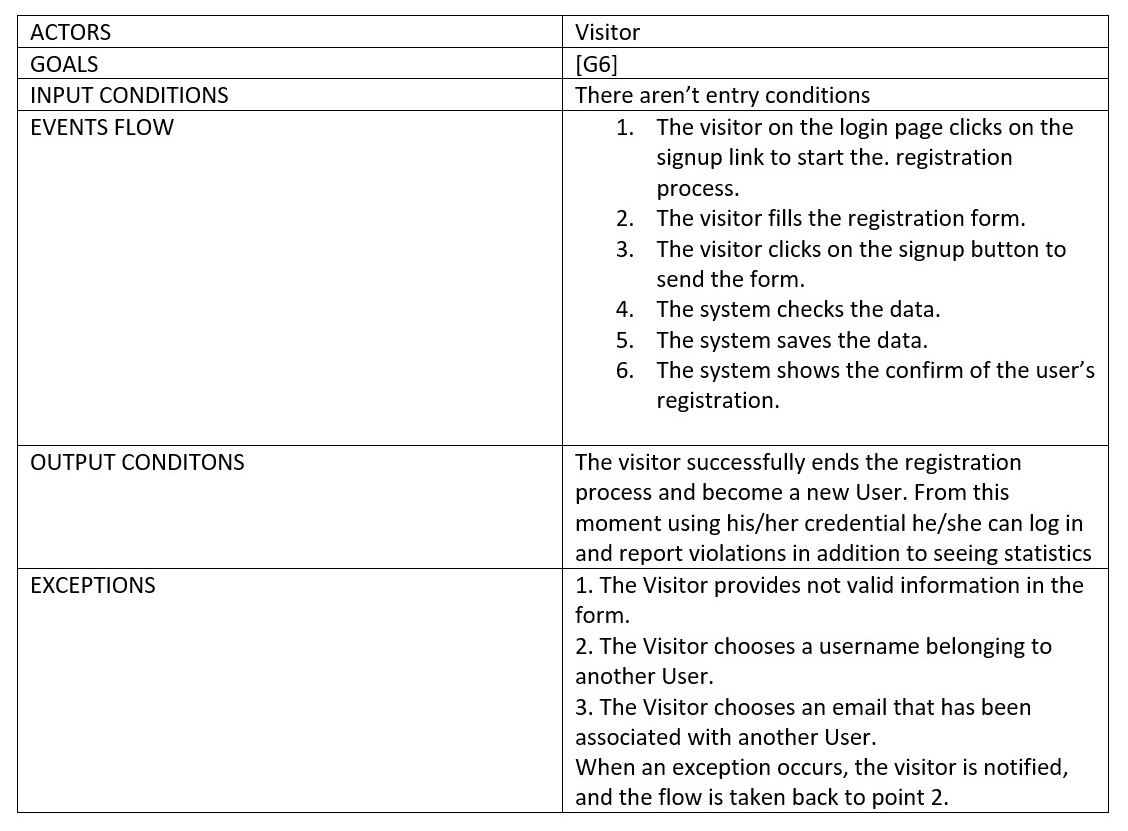
\includegraphics[width=\textwidth]{Images/visitor_use_case.png}
\caption{\label{fig:VUCD}Visitor Use Case Description}
\end{figure}
\begin{figure}[h]
\centering
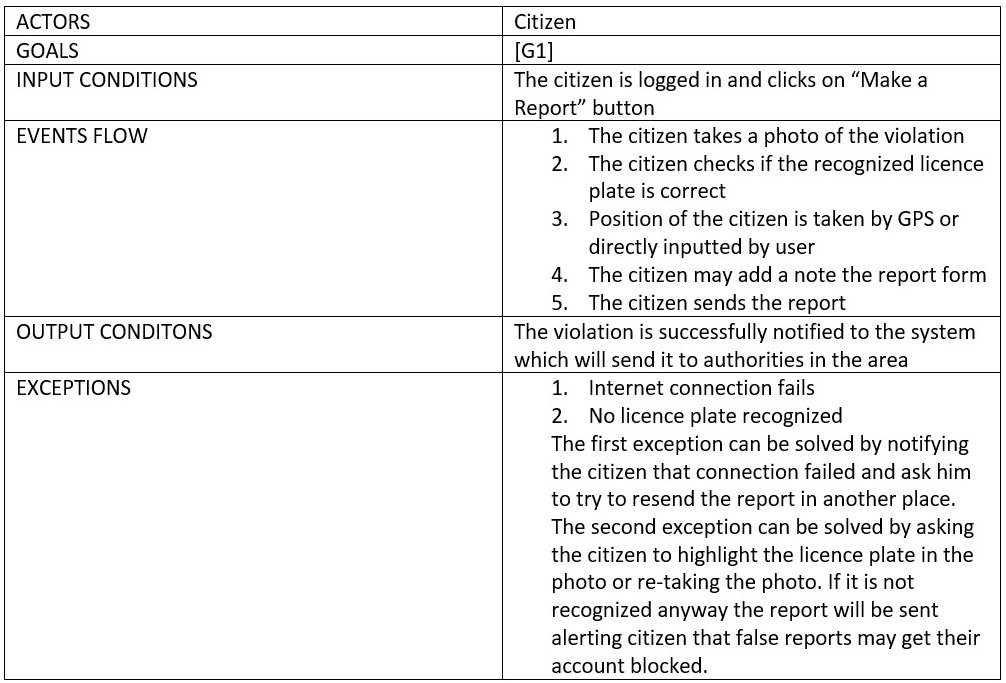
\includegraphics[width=\textwidth]{Images/citizen_use_case.png}
\caption{\label{fig:CUCD}Citizen Use Case Description }
\end{figure}
\begin{figure}[h]
\centering
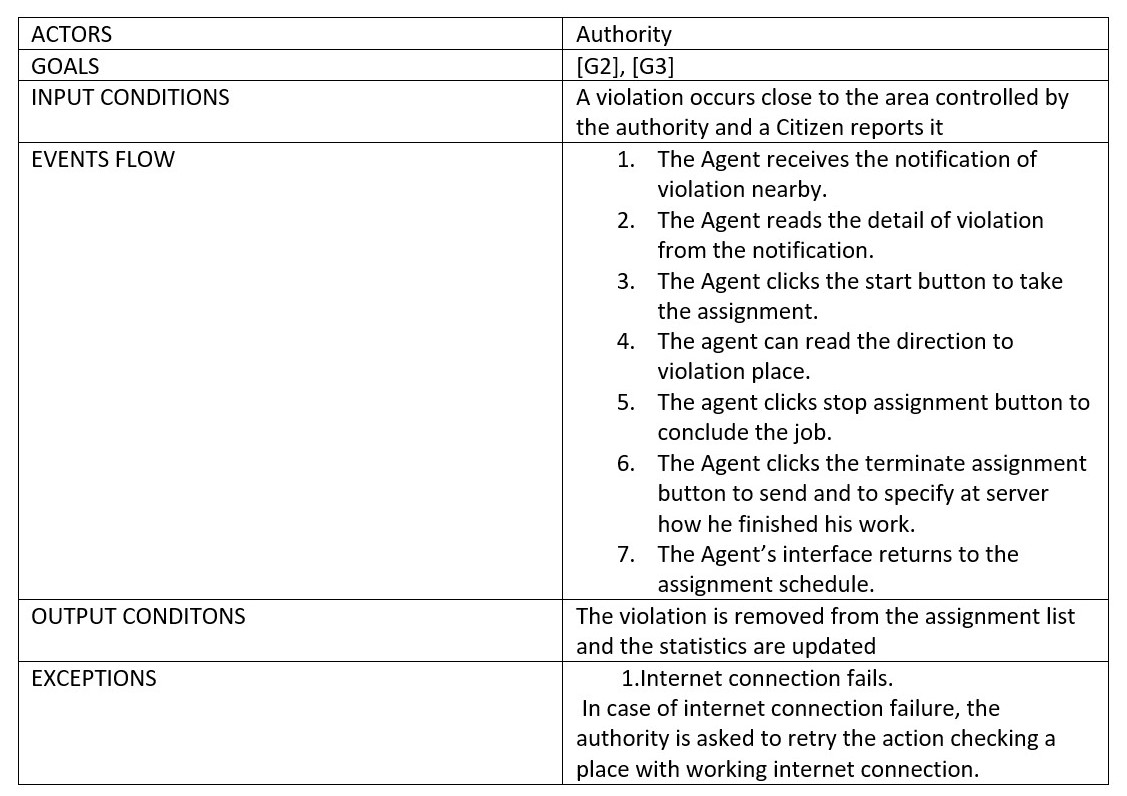
\includegraphics[width=\textwidth]{Images/authority_use_case.png}
\caption{\label{fig:AUCD}Authority Use Case Description 1}
\end{figure}
\begin{figure}[h]
\centering
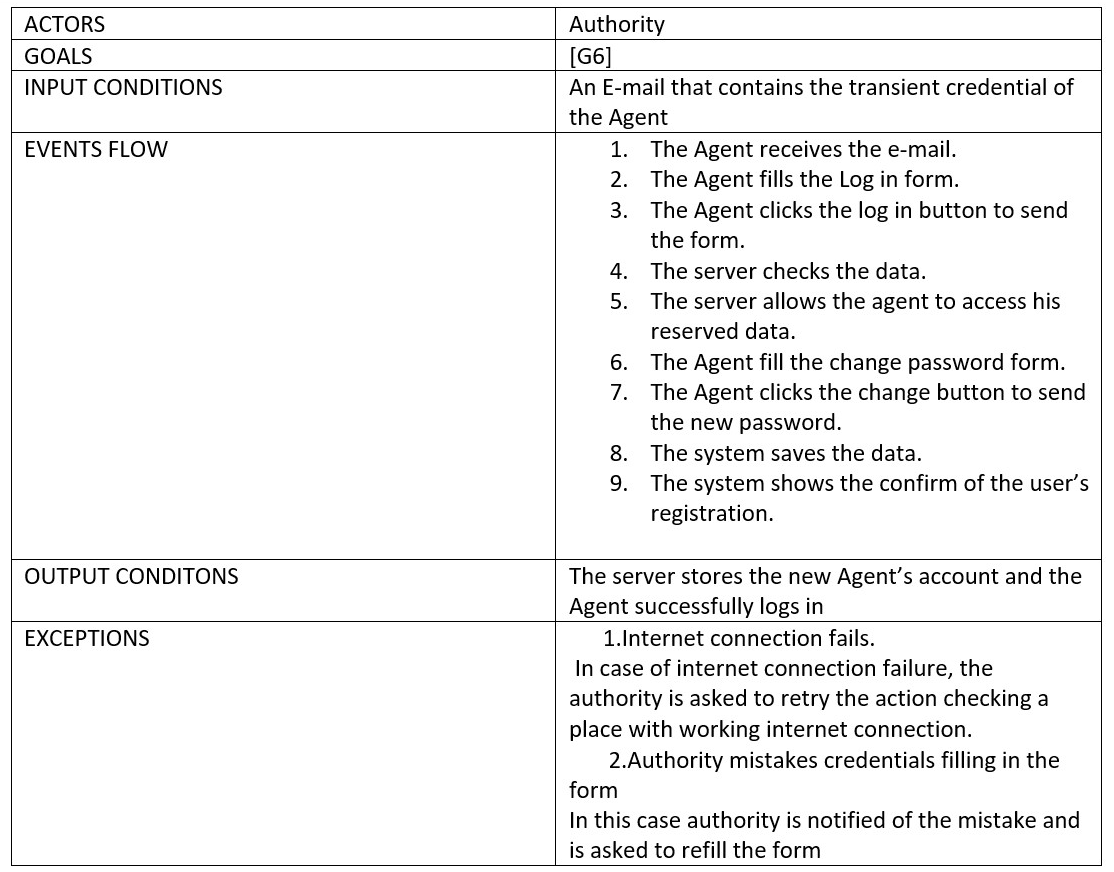
\includegraphics[width=\textwidth]{Images/authority_use_case2.png}
\caption{\label{fig:AUCD2}Authority Use Case Description 2}
\end{figure}
\begin{figure}[h]
\centering
\includegraphics[width=\textwidth]{Images/Municipality_use_case2.png}
\caption{\label{fig:MUCD}Municipality Use Case  Description 1}
\end{figure}
\begin{figure}[h]
\centering
\includegraphics[width=\textwidth]{Images/Municipality_use_case2.png}
\caption{\label{fig:MUCD2}Municipality Use Case  Description 2}
\end{figure}
\begin{figure}[h]
\centering
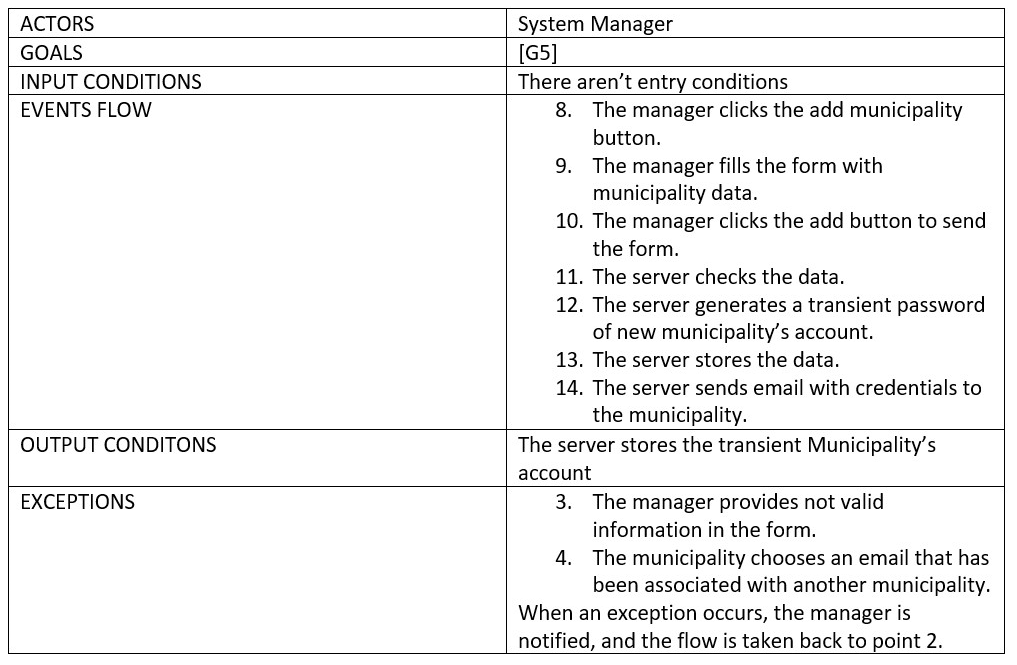
\includegraphics[width=\textwidth]{Images/system_manager_use_case.png}
\caption{\label{fig:SMUCD}System Manager Use Case  Description}
\end{figure}
\begin{figure}[h]
\centering
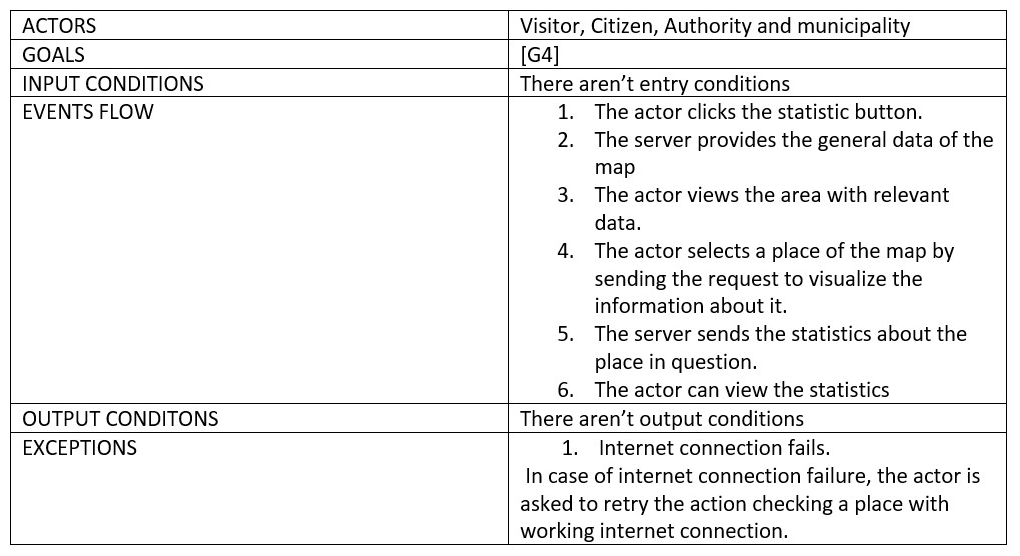
\includegraphics[width=\textwidth]{Images/common_use_case.png}
\caption{\label{fig:CUC}Common Use Case  Description 1} 
\end{figure}
\begin{figure}[h]
\centering
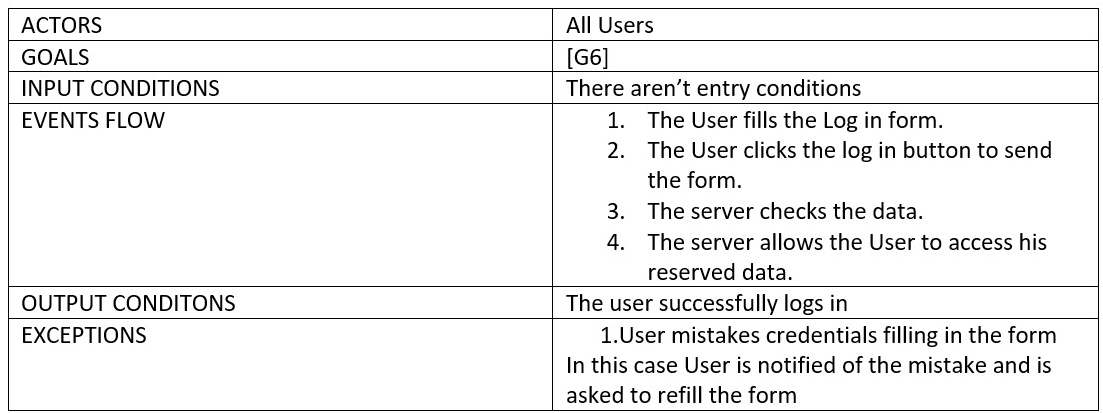
\includegraphics[width=\textwidth]{Images/common_use_case2.png}
\caption{\label{fig:CUC2}Common Use Case  Description 2}
\end{figure}
%.-------------------------------------------------------------------------------------------------------------------------------------------------------------
\subsubsection{Sequence  Diagrams}
\begin{figure}[h]
\centering
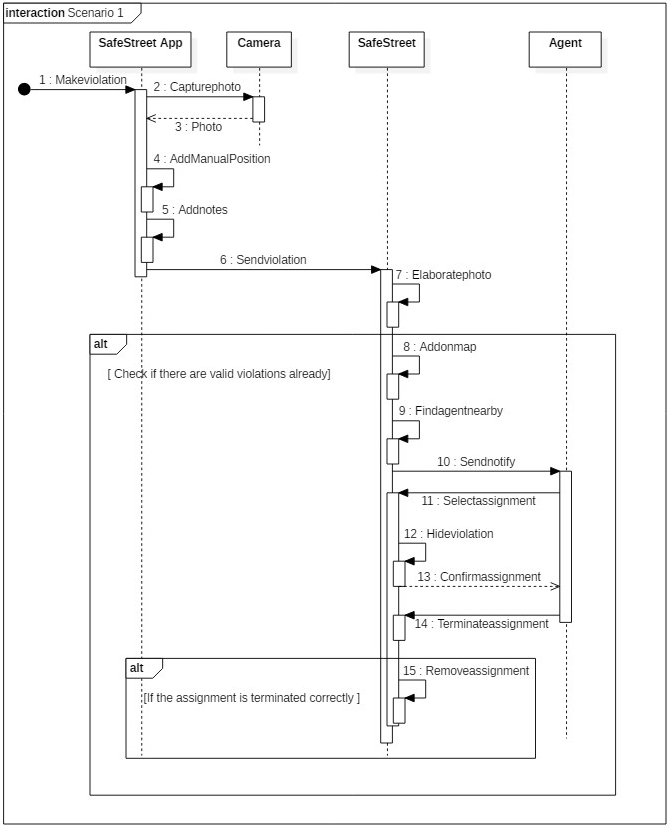
\includegraphics{Images/sequence_scenario1.png}
\caption{\label{fig:SDS1}Sequence Diagram Scenario 1}
\end{figure}
\begin{figure}[h]
\centering
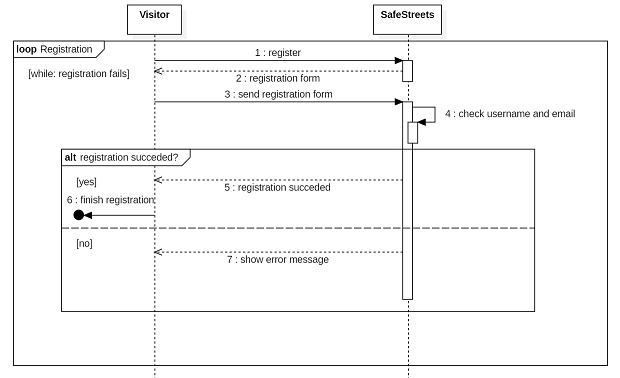
\includegraphics{Images/sequence_registration.png}
\caption{\label{fig:SR} Sequence Diagram Registration}
\end{figure}
\begin{figure}[h]
\centering
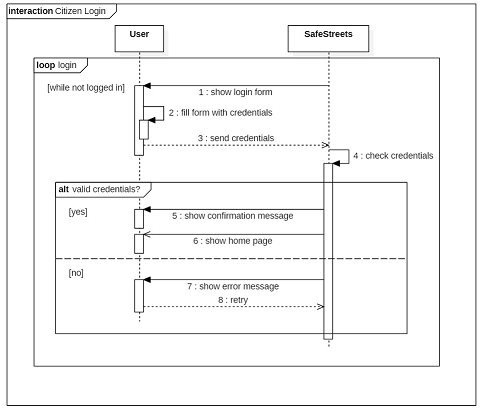
\includegraphics{Images/sequence_login.png}
\caption{\label{fig:SDL}Sequence Diagram Login}
\end{figure}
\begin{figure}[h]
\centering
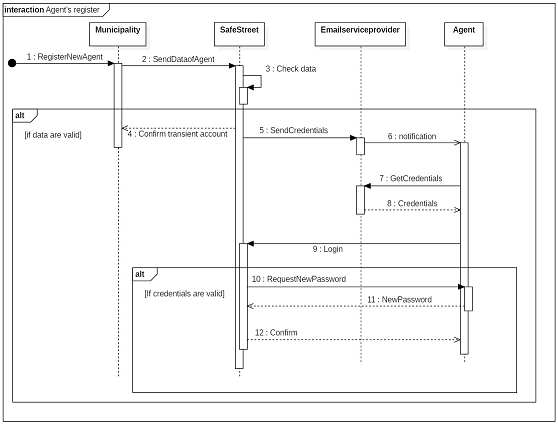
\includegraphics{Images/sequence_agent_register.png}
\caption{\label{fig:SDAR}Sequence Diagram Agent Registrtion} 
\end{figure}

%.-------------------------------------------------------------------------------------------------------------------------------------------------------------
\subsubsection{Mapping of Requirements and Domain Assumptions to their relative goal}
\begin{itemize}
\item G1) Notify authorities about traffic violations
\begin{itemize}
 \item R1) Authorities’ location must be known by the system when they are in service
 \item R2) When a Citizen makes a report the position is correctly added with the GPS when is available.
 \item R3) The right authorities are notified about violations.
 \item R10) When GPS is not available the user can input the position from a map.
 \item D1) For each notification data and metadata provided by the system of the mobile phone are
correct.
 \item D3) GPS of authorities devices works correctly and gives the correct position every time.
 \item D4) Authorities if available correctly informs the system about their availability.
\end{itemize}
\item G2) Authorities must be able to take an available assignment
\begin{itemize}
 \item R1) Authorities’ location must be known by the system when they are in service.
 \item R3) The right authorities are notified about violations.
 \item D3) GPS of authorities devices works correctly and gives the correct position every time.
 \item D4) Authorities if available correctly informs the system about their availability.
 \item D6) System Manager, Municipality and authorities respects their duty of care.
\end{itemize}
\item G3) Allow authorities to report a finished assignment
\begin{itemize}
 \item R4) Authority must be able to provide the system how the assignment finished: resolved and the
type of violation, no intervention needed when arrived, false report.
 \item D6) System Manager, Municipality and authorities respects their duty of care
 \item D8) Information provided by authority are correct and no false report is ignored.
\end{itemize}
\item G4) Allow all actors to visualize updated statistics
\begin{itemize}
\item R5) The system must make Statistics available when asked.
\item R6) Statistics are always updated when an event happens.
 \item D8) Information provided by authority are correct and no false report is ignored.
\end{itemize}
\item G5) Allow the system manager to register Municipality to the service
\begin{itemize}
\item R7) For registering a Municipality his/hers data must be provided to a System manager who will add those data to the service to sign up him/her.
\item R9) When the creation of an account is successful the system must notify the Visitor sending an email to the address provided in the sign up process.
\item D6) System Manager, Municipality and authorities respects their duty of care
\end{itemize}
\item G6) Allow a Visitor to join the system registering him/herself to ensure reliability of the information provided by him/her
\begin{itemize}
\item R8) A visitor must be able to begin sign up process in the SafeStreets App filling a form with his
data.
\item R9) When the creation of an account is successful the system must notify the Visitor sending an
email to the address provided in the sign up process.
 \item R15) Each Username is unique
\end{itemize}
\item G7) Store information about violations provided by users:
\begin{itemize}
 \item R2) When a Citizen makes a report the position is correctly added with the GPS when is available.
 \item R4) Authority must be able to provide the system how the assignment finished: resolved and the
type of violation, no intervention needed when arrived, false report.
 \item R10) When GPS is not available the user can input the position from a map.
 \item R12) The camera of the mobile phone must be accessible to take photos of violations.
 \item R14) The User must be able to select the licence plate between the ones in output from the Licence
Plate Recognition algorithm.
 \item D8) Information provided by authority are correct and no false report is ignored.

\end{itemize}
\item G8) Identify potentially unsafe areas:
\begin{itemize}
\item R4) Authority must be able to provide the system how the assignment finished: resolved and the
type of violation, no intervention needed when arrived, false report.
\item R6) Statistics are always updated when an event happens.
\item D1) For each notification data and metadata provided by the system of the mobile phone are
correct
\item D8) Information provided by authority are correct and no false report is ignored.

\end{itemize}
\item G9) Allow municipality to register Authorities to the service
\begin{itemize}
\item R9) When the creation of an account is successful the system must notify the Visitor sending an
email to the address provided in the sign up process.
\item D6) System Manager, Municipality and authorities respects their duty of care
\item D7) When an authority is sent an email to register this will surely be received
\item D9) The Agent and municipality must be able to communicate
\item D10) Information of authority which is being registered are known by municipality
\end{itemize}
\end{itemize}

%.-------------------------------------------------------------------------------------------------------------------------------------------------------------
\subsection{Performance Requirements}
The system should be able to respond to a possibly great number of simultaneous requests. Based on 
data about Milan, there are over 100.000 parking violations a day, so the system should be able to keep 
track of at least 10 times that number of notifications a day. In some special cases, like public transport 
strikes, the number of violations could increase sensibly and the server could have to manage a lot of 
requests.

%.-------------------------------------------------------------------------------------------------------------------------------------------------------------
\subsection{Design Constraints}
%.-------------------------------------------------------------------------------------------------------------------------------------------------------------
\subsubsection{Standards compliance }
SafeStreets aims to become the smartest and quickest way to report violations in Italy. 
Nowadays, citizens who want to send a report can contact the authorities by calling an emergency number, 
but this can take a lot of time. Moreover, during critical events, phone lines could be unavailable. 
You can also use police website, but its interface is not user-friendly. In any case, you can’t send any 
evidence of the violation to the authorities. Anyway, the idea of our service is not unique: there are already 
similar services in other countries, like in India where there is “Public Eye. OFFICIAL BTP APP”.
%.-------------------------------------------------------------------------------------------------------------------------------------------------------------
\subsubsection{Hardware limitations}
\begin{itemize}
\item Mobile App
\begin{itemize}
\item Android smartphone
\item 2G/3G/4G connection
\item GPS
\end{itemize}
\item Web App
\begin{itemize}
\item Modern browser able to retrieve user's location
\end{itemize}
\end{itemize}
%.-------------------------------------------------------------------------------------------------------------------------------------------------------------
\subsection{Software System Attributes}
%.-------------------------------------------------------------------------------------------------------------------------------------------------------------
\subsubsection{Availability}
The system should be available 99,99\% of time. Considering only one State, there will be a time range 
in which notifications are considerably reduced (the night-time when citizen will less likely report 
a violation) and so reliability constraint for night-time could be reduced up to 99\% reducing also some 
resources allocated to the system.
%.-------------------------------------------------------------------------------------------------------------------------------------------------------------
\subsubsection{Reliability}
There are no strict costraints of Reliability if Availability costraints are respected
%.-------------------------------------------------------------------------------------------------------------------------------------------------------------
\subsubsection{Security}

Users credentials will be stored. Security of the data and of the communications user-system is a primary concern.

%.-------------------------------------------------------------------------------------------------------------------------------------------------------------
\subsubsection {Maintainability}
The system must be developed in a modular way so that new feature can be added.
Using a modular approach it is also possible to test the functionality of the single parts making it simpler to maintain.
Documentation must be also always updated in case of modifications of the system to always keep documentation aligned to the system.
%.-------------------------------------------------------------------------------------------------------------------------------------------------------------
\subsubsection{Scalability}
This system is designed to be optimized in Italy. It is possible to expand it later by choosing a more suitable
algorithm to recognize licence plates and by dividing computation of different states on different servers, so that reliability analysis made for Italy are still true for every single state. Information about boundaries
of states should be replicated in both states making the transition from one server to the other smoother.
%.-------------------------------------------------------------------------------------------------------------------------------------------------------------
\subsubsection{Accuracy}
Accuracy of the position of authorities and violations has to be the best possible. All the sensors used must provide positions' data with an error lower than 20 meters. We can consider a larger bound of accuracy because authorities work on a given area so from a well taken photo, they should be able to recognize the place of the violation even if the position given by the GPS is not too accurate.










